\documentclass[areasetadvanced]{scrartcl}

\usepackage[utf8]{inputenc}
\usepackage[T2A]{fontenc}
\usepackage[english,russian]{babel}

\usepackage[footskip=1cm,left=25mm, right=15mm, top=20mm, bottom=20mm]{geometry}
\usepackage{setspace}
\usepackage{amsmath, amssymb}  % Объединено в одну строку
\usepackage{graphicx}
\usepackage{tikz}
\usetikzlibrary{arrows.meta}
\usepackage{float}
\usepackage{dashrule}
\usepackage{fancyhdr} % оформление отчёта
\usepackage{hyperref} % оформление отчёта
\usepackage{parskip}
\usepackage{textcomp, enumitem}
\usepackage{indentfirst}
\usepackage{hyperref}
\usepackage{graphicx}
\usepackage{algorithm}
\usepackage{algpseudocode}
\usepackage{array}  % Для использования команды m{}
\usepackage{geometry}
\usepackage{afterpage}
\usepackage{minted}
\setcounter{secnumdepth}{3}  % Включает нумерацию для subsubsection
\setcounter{tocdepth}{3}     % Включает subsubsection в содержание
\usepackage{listings} % Если используете listings

\tikzstyle{block} = [rectangle, rounded corners, minimum width=3cm, minimum height=1cm, text centered, draw=black, fill=lightgray]

\setkomafont{sectioning}{\normalfont\bfseries} % для заголовков разделов и подразделов
\setkomafont{section}{\normalfont\Large\bfseries}
\setkomafont{subsection}{\normalfont\large\bfseries}
\setkomafont{subsubsection}{\normalfont\large\bfseries}
\setkomafont{paragraph}{\normalfont\large\bfseries} % для заголовков параграфов (если они есть)

\lstset{
  language=Python,
  basicstyle=\ttfamily\small,
  keywordstyle=\color{blue}\bfseries,
  stringstyle=\color{red},
  commentstyle=\color{green!70!black},
  numbers=left,
  numberstyle=\tiny,
  stepnumber=1,
  numbersep=10pt,
  showstringspaces=false,
  breaklines=true,
  frame=single
}

\setcounter{tocdepth}{2}
\begin{document}
\sloppy
	\thispagestyle{empty}
	\begin{center}
		\large{МИНОБРНАУКИ РОССИИ} \par
		\vspace{0.3cm}
		\normalsize
		{ФЕДЕРАЛЬНОЕ ГОСУДАРСТВЕННОЕ АВТОНОМНОЕ ОБРАЗОВАТЕЛЬНОЕ УЧРЕЖДЕНИЕ ВЫСШЕГО ОБРАЗОВАНИЯ} \par
		\vspace{0.3cm}
		\textbf{\guillemotleft САНКТ-ПЕТЕРБУРГСКИЙ ПОЛИТЕХНИЧЕСКИЙ}
		\textbf{УНИВЕРСИТЕТ ПЕТРА ВЕЛИКОГО\guillemotright} \par
		\vspace{0.3cm}
		{Институт компьютерных наук и кибербезопасности}\par
		{Высшая школа технологий искусственного интеллекта}\par
	\end{center}
	\vfill
	\begin{center}
		{\large Отчёт по дисциплине \guillemotleft Сети ЭВМ и телекоммуникации компьютерных сетей\guillemotright}\par
		{\huge   Лабораторная работа №3
		
		\guillemotleft AMQP протокол и брокер сообщений\guillemotright}\par
            {\huge Вариант \textbf{№9}}
         
	\end{center}
	\vfill
	\begin{flushleft}
		Студент: \hspace{1.8cm} \rule[0pt]{2.5cm}{0.5pt}\hfill Салимли Айзек Мухтар Оглы\par
		\vspace{1.5cm}
		Преподаватель: \hspace{0.55cm} \rule[0pt]{2.5cm}{0.5pt}\hfill  Мулюха Владимир Александрович
	\end{flushleft}
	\vspace{0.5cm}
	\begin{flushright}
		\guillemotleft \rule[0pt]{0.8cm}{0.5pt}\guillemotright \rule[0pt]{2cm}{0.5pt} 20\rule[0pt]{0.5cm}{0.5pt} г.
	\end{flushright}
	\vfill
	\begin{center}
		Санкт-Петербург, 2025
	\end{center}
	\newpage
	\tableofcontents
	\newpage
\section*{Введение}
	\addcontentsline{toc}{section}{Введение}
В данном отчете, приведена и описана реализация, подключения AMQP протокола, с помощью \textbf{RabbitMQ}. 
В лабораторной работе нужно: 
\begin{itemize}
	\item Организовать общение трех отправителей и трех получателей.
	\item Каждому получателю соответсвует своя очередь.
	\item Отправители могут писать в каждую из очередей, используя механизм Header Exchange с различными комбинациями полей.
\end{itemize}

Для выполнения работы, был написан код на языке Python 3.13.2, в среде разработки VSCode, с использованием библиотеки \textbf{pika}.
Было созданно два .py файла:
\begin{itemize}
	\item sender.py \# Отправитель
	\item receiver.py \# Получатель
\end{itemize}

Для сборки контейнера был использован Docker:
\begin{itemize}
	\item Dockerfile \# Докер-файл для Python с использованием pika
	\item docker-compose.yaml \# Порты и сервисы 
\end{itemize}

\newpage
\section{Постановка задачи}
Используя Docker, создать контейнеры, необходимые для реализации следующего функци-
онала с использованием RabbitMQ, а также показать как именно осуществляется передача
в этих условиях.
Вариант 9. Организовать общение трех отправителей и трех получателей, при этом каждому
получателю соотвествует своя очередь. А отправители могут писать в каждую из очередей,
используя механизм Header Exchange с различными комбинациями полей.

\newpage
\section{AMQP протокол}
%%%%%%%%%%%%%%%%%%%%%%%%%%%
Открытый протокол прикладного уровня для передачи сообщений между компонентами системы. Основная идея состоит в том, что отдельные подсистемы (или независимые приложения) могут обмениваться произвольным образом сообщениями через AMQP-брокер, который осуществляет маршрутизацию, возможно гарантирует доставку, распределение потоков данных, подписку на нужные типы сообщений.

AMQP основан на:
\begin{itemize}
	\item Message — единица передаваемых данных, содержание никак не интерпретируется сервером, к сообщению могут быть присоединены структурированные заголовки
	\item Exchange - в неё отправляются сообщения. Точка обмена распределяет сообщения в одну или несколько очередей. При этом в точке обмена сообщения не хранятся. Точки обмена бывают трёх типов: \begin{itemize}
		\item fanout — сообщение передаётся во все прицепленные к ней очереди
		\item direct — сообщение передаётся в очередь с именем, совпадающим с ключом маршрутизации (routing key) (ключ маршрутизации указывается при отправке сообщения)
		\item topic — нечто среднее между fanout и direct, сообщение передаётся в очереди, для которых совпадает маска на ключ маршрутизации.
	\end{itemize}
\end{itemize}

\subsection{Слои}
Functional Layer - определяет набор команд которые выполняют работу от имени приложения.
Transport Layer - обслуживает запросы приложения к серверу и сервера к приложению, управляет мультиплексированием каналов, фреймингом, кодировкой, heart-beating, представлением данныx, работой с ошибками.

\newpage
\section{Брокер сообщений}
%%%%%%%%%%%%%%%%%%%%%%%%%%%
приложение, которое преобразует сообщение по одному протоколу от приложения-источника в сообщение протокола приложения-приёмника, тем самым выступая между ними посредником. Кроме преобразования сообщений из одного формата в другой, в задачи брокера сообщений также входит:
\begin{itemize} 
	\item проверка сообщения на ошибки
	\item маршрутизация конкретному приемнику(ам)
	\item разбиение сообщения на несколько маленьких, а затем агрегирование ответов приёмников и отправка результата источнику
	\item сохранение сообщений в базе данных
	\item вызов веб-сервисов
	\item распространение сообщений подписчикам, если используются шаблоны типа «издатель — подписчик»
\end{itemize}
Использование брокеров сообщений позвOlyaет разгрузить веб-сервисы в распределённой системе, так как при отправке сообщений им не нужно тратить время на некоторые ресурсоёмкие операции типа маршрутизации и поиска приёмников. Кроме того, брокер сообщений для повышения эффективности может реализовывать стратегии упорядоченной рассылки и определение приоритетности, балансировать нагрузку и прочее.

\newpage
\section{RabbitMQ}
%%%%%%%%%%%%%%%%%%%%%%%%%%%
RabbitMQ поддерживает несколько протоколов, включая AMQP (Advanced Message Queuing Protocol), MQTT (Message Queuing Telemetry Transport), STOMP (Simple Text Oriented Messaging Protocol).

RabbitMQ гарантирует доставку сообщений получателю. Для этого используется механизм подтверждения доставки (Acknowledgements), который позвOlyaет отправителю сообщения быть уверенным в том, что адресат его получил. Если получатель не подтверждает получение сообщения, RabbitMQ автоматически повторяет отправку.

Кроме этого, в RabbitMQ реализована пуш-модель получения сообщений, которая позвOlyaет серверу активно отправлять информацию клиенту без запроса со стороны последнего. Это особенно полезно в ситуациях, когда нужно быстро информировать клиентов о важных событиях или изменениях в системе.

Сущности RabbitMQ:
\begin{itemize}
	\item Очередь (Queue) — это структура данных, где хранятся сообщения до того, как получатель их обработает. Очередь может быть временной или постоянной, в зависимости от потребностей приложения.
	\item Сообщение (Message) — это единица данных, которая передается от издателя к подписчику через очередь. Сообщения могут быть разных типов и форматов.
	\item Обменник (Exchange) — это компонент, который принимает сообщения от издателей и направляет их в соответствующие очереди.
	\item Биндинг (Binding) — это связь между обменником и очередью, которая определяет, какие сообщения в какую очередь будут направлены.
	\item Продюсер (Producer) — это приложение, которое публикует сообщения в обменник
	\item Получатель (Consumer) — это приложение, которое получает сообщения из очереди и обрабатывает их
\end{itemize}

Принцип работы:
\begin{itemize}
	\item продюсер отправляет сообщение в обменник
	\item обменник направляет сообщение в соответствующую очередь, в зависимости от типа обмена и биндинга
	\item получатель подписывается на очередь и начинает получать сообщения из нее
	\item получатель обрабатывает сообщения и выполняет необходимые действия
	\item получатель подтверждает получение сообщения, чтобы исключить его из очереди
	\item если сообщение не было подтверждено в течение определенного времени, оно будет повторно отправлено в очередь
\end{itemize}

\begin{figure}[H]
	\centering
	
\includegraphics[width=0.7\textwidth]{image.png}
	\caption{Схема работы RabbitMQ}
	\label{fig:syntdiag}
\end{figure}

\newpage
\section{Header Exchange}
%%%%%%%%%%%%%%%%%%%%%%%%%%%
Header Exchange - предназначен для маршрутизации нескольких атрибутов, которые легче выразить в виде заголовков сообщений, чем ключ маршрутизации. Обмен заголовками игнорирует атрибут ключа маршрутизации. Вместо этого атрибуты, используемые для маршрутизации, берутся из атрибута заголовков.

\newpage
\section{Программная реализация}
%%%%%%%%%%%%%%%%%%%%%%%%%%%
\subsection{sender.py}
Файл сценария отправки сообщений в Exchange: 
Подключается к брокеру, объявляет Header Exchange пока он не существует, отправляет несколько сообщений с заголовками и завершается.
Тут exchange-type=headers - Exchange обрабатывает сообщения по заголовкам. А в properties - указываются нужные заголовки.
После отправки скрипт закрывает соединение и завершается.

\begin{lstlisting}
import pika
import os
import time

RABBITMQ_HOST = os.environ.get('RABBITMQ_HOST', 'rabbitmq')
params = pika.ConnectionParameters(host=RABBITMQ_HOST)

MAX_RETRIES = 10
SLEEP_BETWEEN = 3  

connection = None
for i in range(MAX_RETRIES):
    try:
        connection = pika.BlockingConnection(params)
        print("Connected to RabbitMQ!")
        break
    except pika.exceptions.AMQPConnectionError as e:
        print(f"Failed to connect to RabbitMQ. Retrying in {SLEEP_BETWEEN} sec...")
        time.sleep(SLEEP_BETWEEN)

if not connection:
    raise Exception("Could not connect to RabbitMQ after several attempts.")

channel = connection.channel()
exchange_name = 'headers_exchange'
channel.exchange_declare(exchange=exchange_name, exchange_type='headers')

sender_id = os.environ.get('SENDER_ID', 'sender1')

messages = [
    {
        'body': f'Message from {sender_id} with header type=report, format=pdf',
        'headers': {'type': 'report', 'format': 'pdf', 'sender': sender_id}
    },
    {
        'body': f'Message from {sender_id} with header region=EU, priority=low',
        'headers': {'region': 'EU', 'priority': 'low', 'sender': sender_id}
    },
    {
        'body': f'Message from {sender_id} with header department=sales, urgency=high',
        'headers': {'department': 'sales', 'urgency': 'high', 'sender': sender_id}
    },
]
for msg in messages:
    properties = pika.BasicProperties(headers=msg['headers'])
    channel.basic_publish(
        exchange=exchange_name,
        routing_key='',
        body=msg['body'],
        properties=properties
    )
    print(f"Sent: {msg['body']} with headers: {msg['headers']}")
    time.sleep(2)
connection.close()
\end{lstlisting}
\subsection{receiver.py}
Сценарий приёма сообщений (прослушивания) из очереди, связанной с тем же Exchange по заголовкам.
Он будет подключатся к RabbitMQ, так же объявит Headers Exchange, и очередь. Связывает очередь с Exchange, указывает критерии заголовков (arguments). Далее потребляет сообщения и выводит на экран если заголовки совподают с критериями.
\begin{lstlisting}
import pika
import os
import json
import time

RABBITMQ_HOST = os.environ.get('RABBITMQ_HOST', 'rabbitmq')
QUEUE_NAME = os.environ.get('QUEUE_NAME', 'queue1')

MAX_RETRIES = 10
SLEEP_BETWEEN = 3

connection = None
for attempt in range(MAX_RETRIES):
    try:
        params = pika.ConnectionParameters(host=RABBITMQ_HOST)
        connection = pika.BlockingConnection(params)
        print("Connected to RabbitMQ!")
        break
    except pika.exceptions.AMQPConnectionError:
        print(f"Failed to connect to RabbitMQ. Retrying in {SLEEP_BETWEEN} seconds... (Attempt {attempt+1}/{MAX_RETRIES})")
        time.sleep(SLEEP_BETWEEN)

if not connection:
    raise Exception(f"Could not connect to RabbitMQ after {MAX_RETRIES} attempts")

channel = connection.channel()

exchange_name = 'headers_exchange'
channel.exchange_declare(exchange=exchange_name, exchange_type='headers')
channel.queue_declare(queue=QUEUE_NAME)

binding_criteria = os.environ.get('BINDING_CRITERIA', '{}')
try:
    binding_args = json.loads(binding_criteria)
except json.JSONDecodeError:
    binding_args = {}
    
channel.queue_bind(queue=QUEUE_NAME, exchange=exchange_name, arguments=binding_args)
print(f"Receiver listening on queue '{QUEUE_NAME}' with binding criteria: {binding_args}")

def callback(ch, method, properties, body):
    print(f"Received in '{QUEUE_NAME}': {body.decode()} with headers: {properties.headers}")

channel.basic_consume(queue=QUEUE_NAME, on_message_callback=callback, auto_ack=True)

print("Starting consuming...")
channel.start_consuming()

\end{lstlisting}

\subsection{Dockerfile}
Инструкция для создания Docker-образа, содержащего Python-приложение. У каждого .py файла свой Dockerfile: для sender и receiver.
Описывает, как собрать Docker-образ для вашего Python-приложения (как отправителя, так и получателя).
Содержит базовый образ python:3.9, устанавливает необходимые зависимости (например, pika), копирует нужные .py файлы и задаёт команду по умолчанию.
\begin{lstlisting}
FROM python:3.9
WORKDIR /app
COPY sender.py .
RUN pip install pika
CMD ["python", "sender.py"]
\end{lstlisting}
\subsection{docker-compose.yaml}
\begin{itemize}
	\item Файл, управляющий запуском всех сервисов в контейнерах: RabbitMQ, отправители, получатели, и задающий их связь.
	\item Запускает все сервисы в контейнерах (RabbitMQ, несколько отправителей, несколько получателей).
	\item Описывает, какие образы (или сборки) запускать, какие порты мапить, какие переменные окружения передавать и т.д.
	\item Раздел services: перечисляет, например, rabbitmq, sender1, sender2, receiver1, и т.д.
	\item Для rabbitmq обычно указывается образ rabbitmq:3-management и порты 5672 (AMQP) и 15672 (панель управления).
	\item \text{build: ./sender или build: ./receiver – пути к контексту сборки Docker.}
	\item environment: – переменные окружения для Python-кода (например, RABBITMQ HOST, BINDING CRITERIA).
	\item depends-on: – указывает, что отправители или получатели должны запускаться после того, как запустится RabbitMQ 
\end{itemize}
\begin{lstlisting}
version: '3.8'
services:
  rabbitmq:
    image: rabbitmq:3-management
    container_name: rabbitmq
    ports:
      - "5672:5672"
      - "15672:15672"

  sender1:
    build:
      context: ./sender      
    container_name: sender_ayzek
    environment:
      SENDER_ID: "Ayzek"
      RABBITMQ_HOST: rabbitmq
    depends_on:
      - rabbitmq

  sender2:
    build:
      context: ./sender      
    container_name: sender_petya
    environment:
      SENDER_ID: "Petya"
      RABBITMQ_HOST: rabbitmq
    depends_on:
      - rabbitmq

  sender3:
    build:
      context: ./sender
    container_name: sender_vasya
    environment:
      SENDER_ID: "Vasya"
      RABBITMQ_HOST: rabbitmq
    depends_on:
      - rabbitmq

  receiver1:
    build:
      context: ./receiver    
    container_name: receiver_masha
    environment:
      QUEUE_NAME: "queueMasha"
      RABBITMQ_HOST: rabbitmq
      BINDING_CRITERIA: '{"x-match": "all", "type": "report", "format": "pdf"}'
    depends_on:
      - rabbitmq

  receiver2:
    build:
      context: ./receiver
    container_name: receiver_olya
    environment:
      QUEUE_NAME: "queueOlya"
      RABBITMQ_HOST: rabbitmq
      BINDING_CRITERIA: '{"x-match": "any", "region": "EU", "priority": "low"}'
    depends_on:
      - rabbitmq

  receiver3:
    build:
      context: ./receiver
    container_name: receiver_misha
    environment:
      QUEUE_NAME: "queueMisha"
      RABBITMQ_HOST: rabbitmq
      BINDING_CRITERIA: '{"x-match": "all", "department": "sales"}'
    depends_on:
      - rabbitmq

\end{lstlisting}

\newpage
\section{Результаты (консоль)}
%%%%%%%%%%%%%%%%%%%%%%%%%%%
\begin{lstlisting}
sender_petya    | Connected to RabbitMQ!
sender_petya    | Sent: Message from Petya with header type=report, format=pdf with headers: {'type': 'report', 'format': 'pdf', 'sender': 'Petya'}
sender_petya    | Sent: Message from Petya with header region=EU, priority=low with headers: {'region': 'EU', 'priority': 'low', 'sender': 'Petya'}
rabbitmq        | 2025-04-15 18:31:13.027586+00:00 [info] <0.697.0> closing AMQP connection <0.697.0> (172.18.0.8:59700 -> 172.18.0.2:5672, vhost: '/', user: 'guest')
sender_petya    | Sent: Message from Petya with header department=sales, urgency=high with headers: {'department': 'sales', 'urgency': 'high', 'sender': 'Petya'}
sender_ayzek    | Failed to connect to RabbitMQ. Retrying in 3 sec...
sender_ayzek    | Failed to connect to RabbitMQ. Retrying in 3 sec...
rabbitmq        | 2025-04-15 18:31:13.059614+00:00 [info] <0.748.0> closing AMQP connection <0.748.0> (172.18.0.6:50664 -> 172.18.0.2:5672, vhost: '/', user: 'guest')
sender_ayzek    | Connected to RabbitMQ!
sender_ayzek    | Sent: Message from Ayzek with header type=report, format=pdf with headers: {'type': 'report', 'format': 'pdf', 'sender': 'Ayzek'}
sender_ayzek    | Sent: Message from Ayzek with header region=EU, priority=low with headers: {'region': 'EU', 'priority': 'low', 'sender': 'Ayzek'}
sender_ayzek    | Sent: Message from Ayzek with header department=sales, urgency=high with headers: {'department': 'sales', 'urgency': 'high', 'sender': 'Ayzek'}
sender_vasya    | Failed to connect to RabbitMQ. Retrying in 3 sec...
sender_vasya    | Failed to connect to RabbitMQ. Retrying in 3 sec...
sender_vasya    | Connected to RabbitMQ!
sender_vasya    | Sent: Message from Vasya with header type=report, format=pdf with headers: {'type': 'report', 'format': 'pdf', 'sender': 'Vasya'}
sender_vasya    | Sent: Message from Vasya with header region=EU, priority=low with headers: {'region': 'EU', 'priority': 'low', 'sender': 'Vasya'}
rabbitmq        | 2025-04-15 18:31:13.070962+00:00 [info] <0.761.0> closing AMQP connection <0.761.0> (172.18.0.7:49862 -> 172.18.0.2:5672, vhost: '/', user: 'guest')
sender_vasya    | Sent: Message from Vasya with header department=sales, urgency=high with headers: {'department': 'sales', 'urgency': 'high', 'sender': 'Vasya'}
sender_petya exited with code 0
sender_vasya exited with code 0
sender_ayzek exited with code 0
Gracefully stopping... (press Ctrl+C again to force)
[+] Stopping 7/7
\end{lstlisting}
\newpage
\section{Результаты (localhost)}
Для запуска используется localhost 15672 как стандарт для панели управления. После чего открывается страница RabbitMQ, где нужно ввести:
\begin{itemize}
	\item Login: guest
	\item Password: guest
\end{itemize}
На рисунках 2-5 показаны графические результаты.
%%%%%%%%%%%%%%%%%%%%%%%%%%%
\begin{figure}[H]
	\centering
	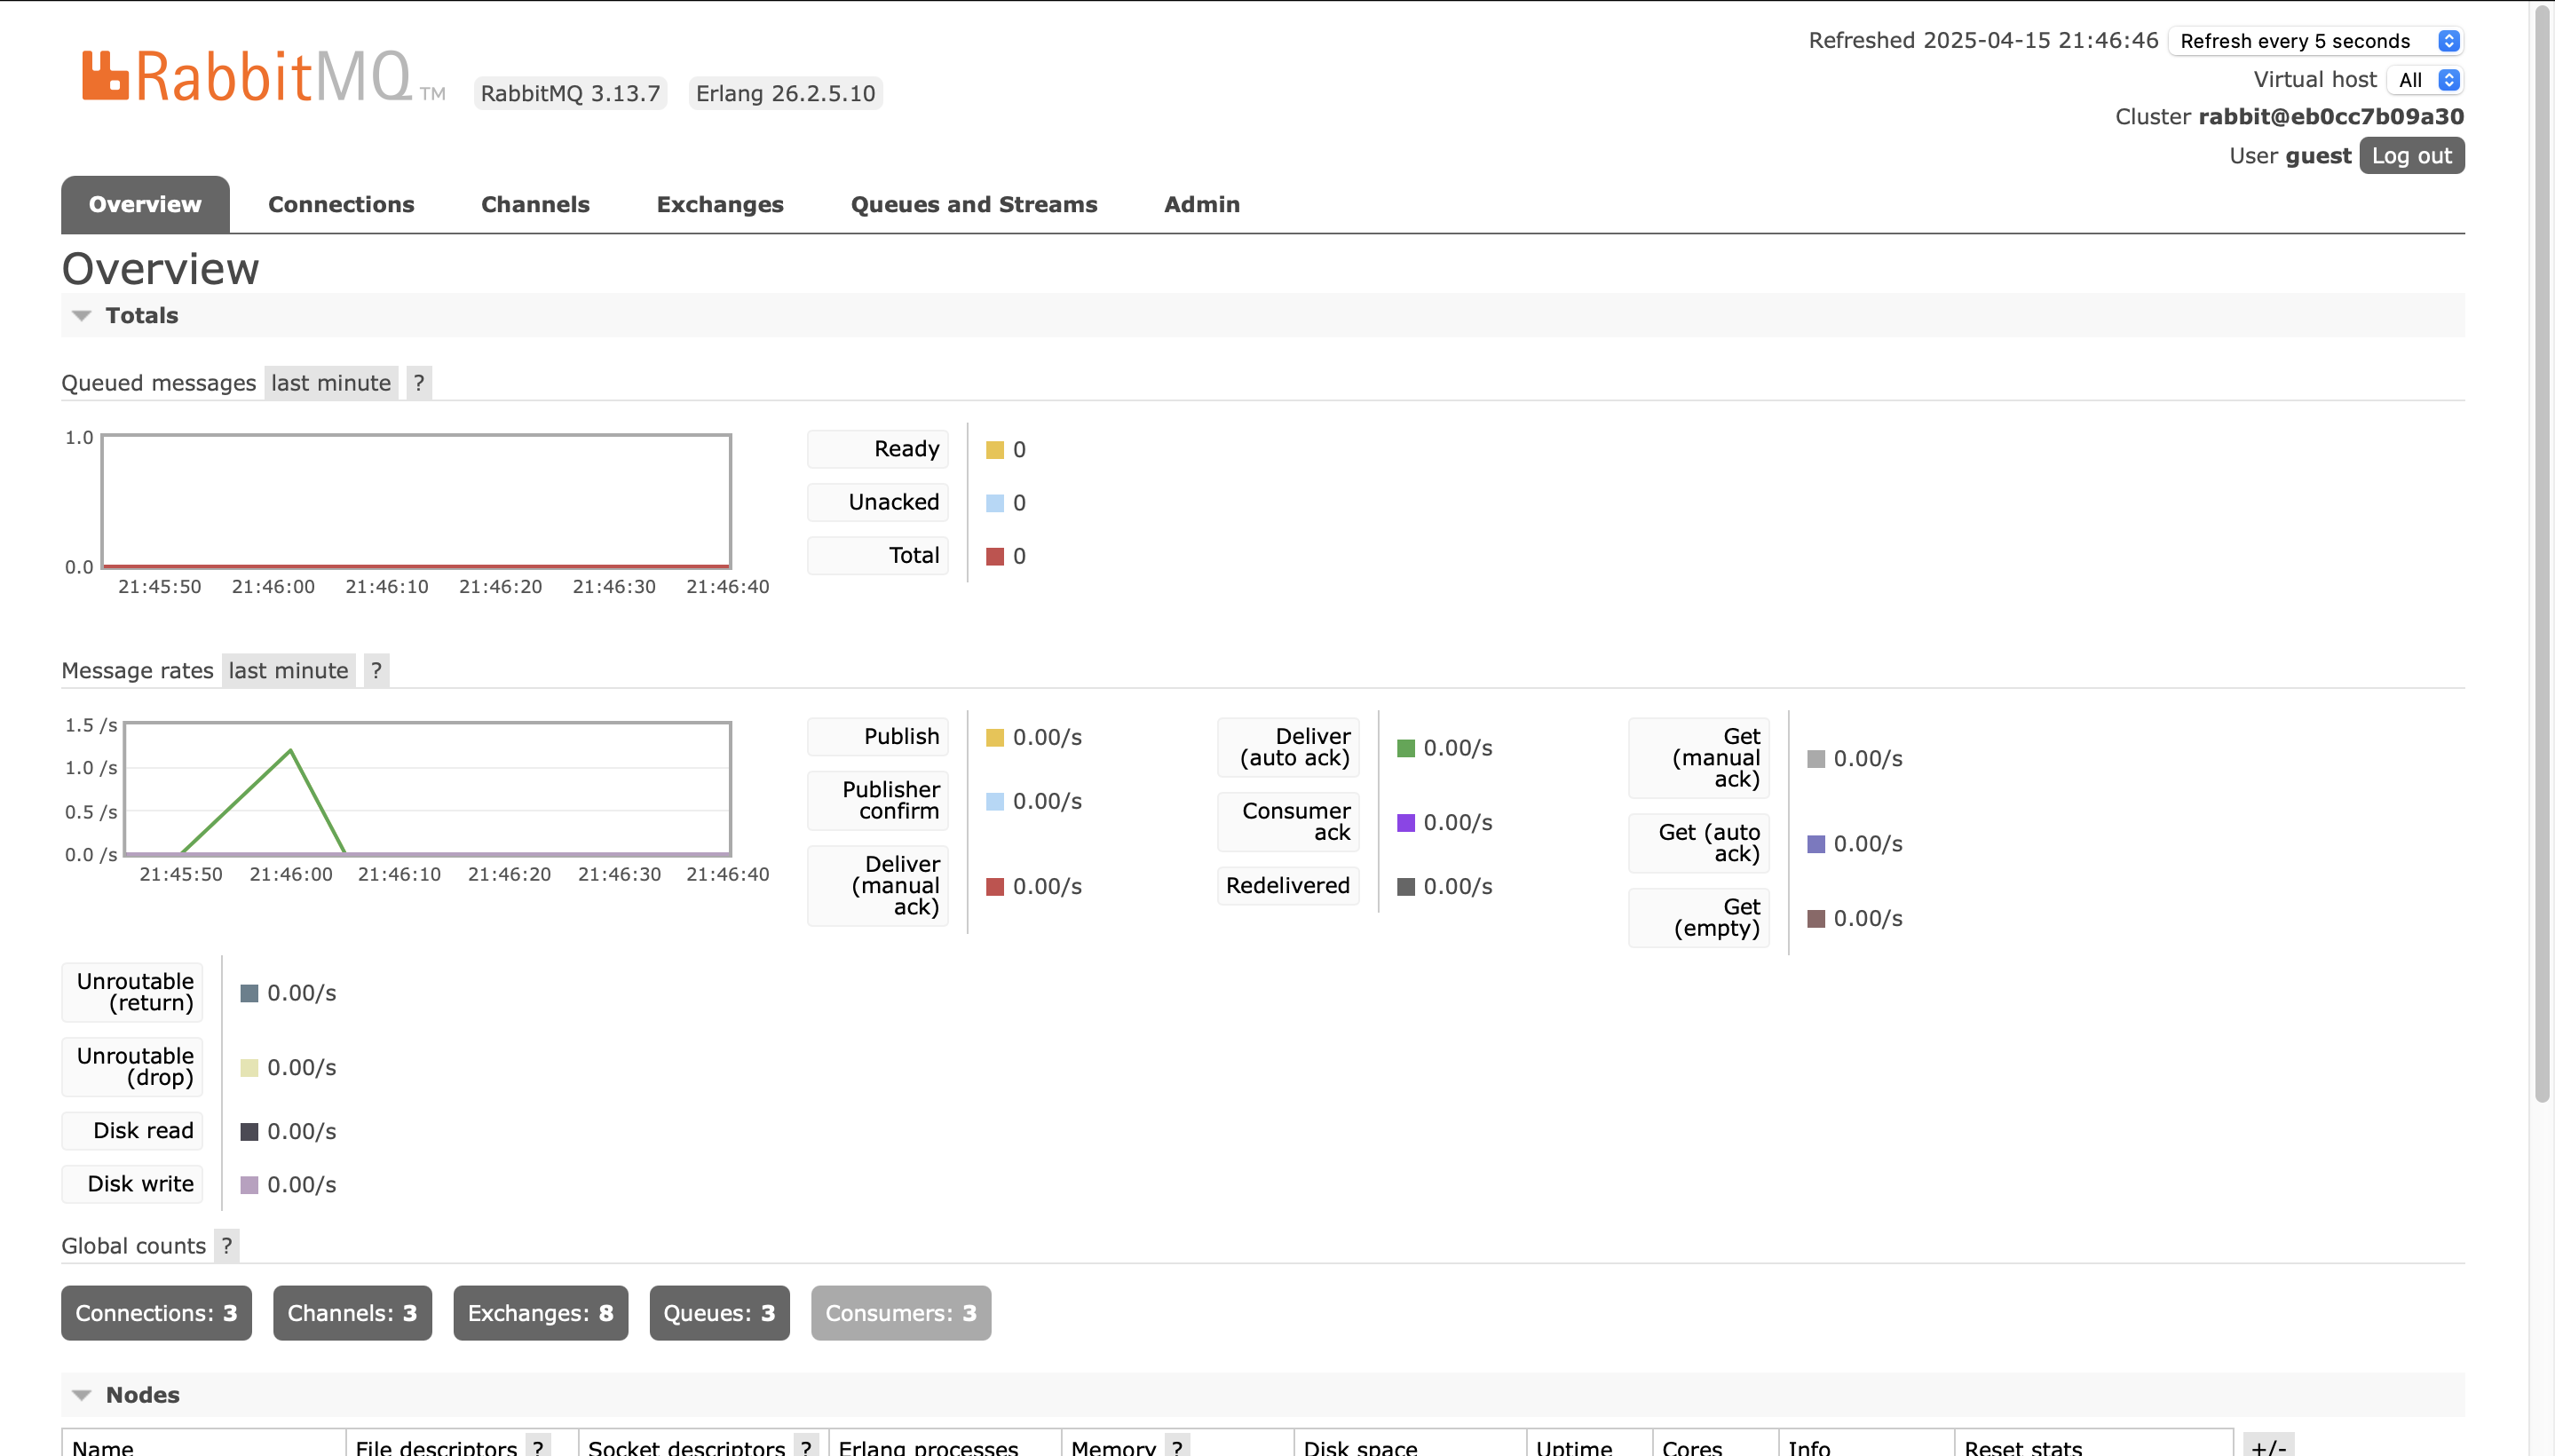
\includegraphics[width=0.7\textwidth]{Overview.png}
	\caption{Краткий обзор RabbitMQ}
	\label{fig:syntdiag}
\end{figure}

\begin{figure}[H]
	\centering
	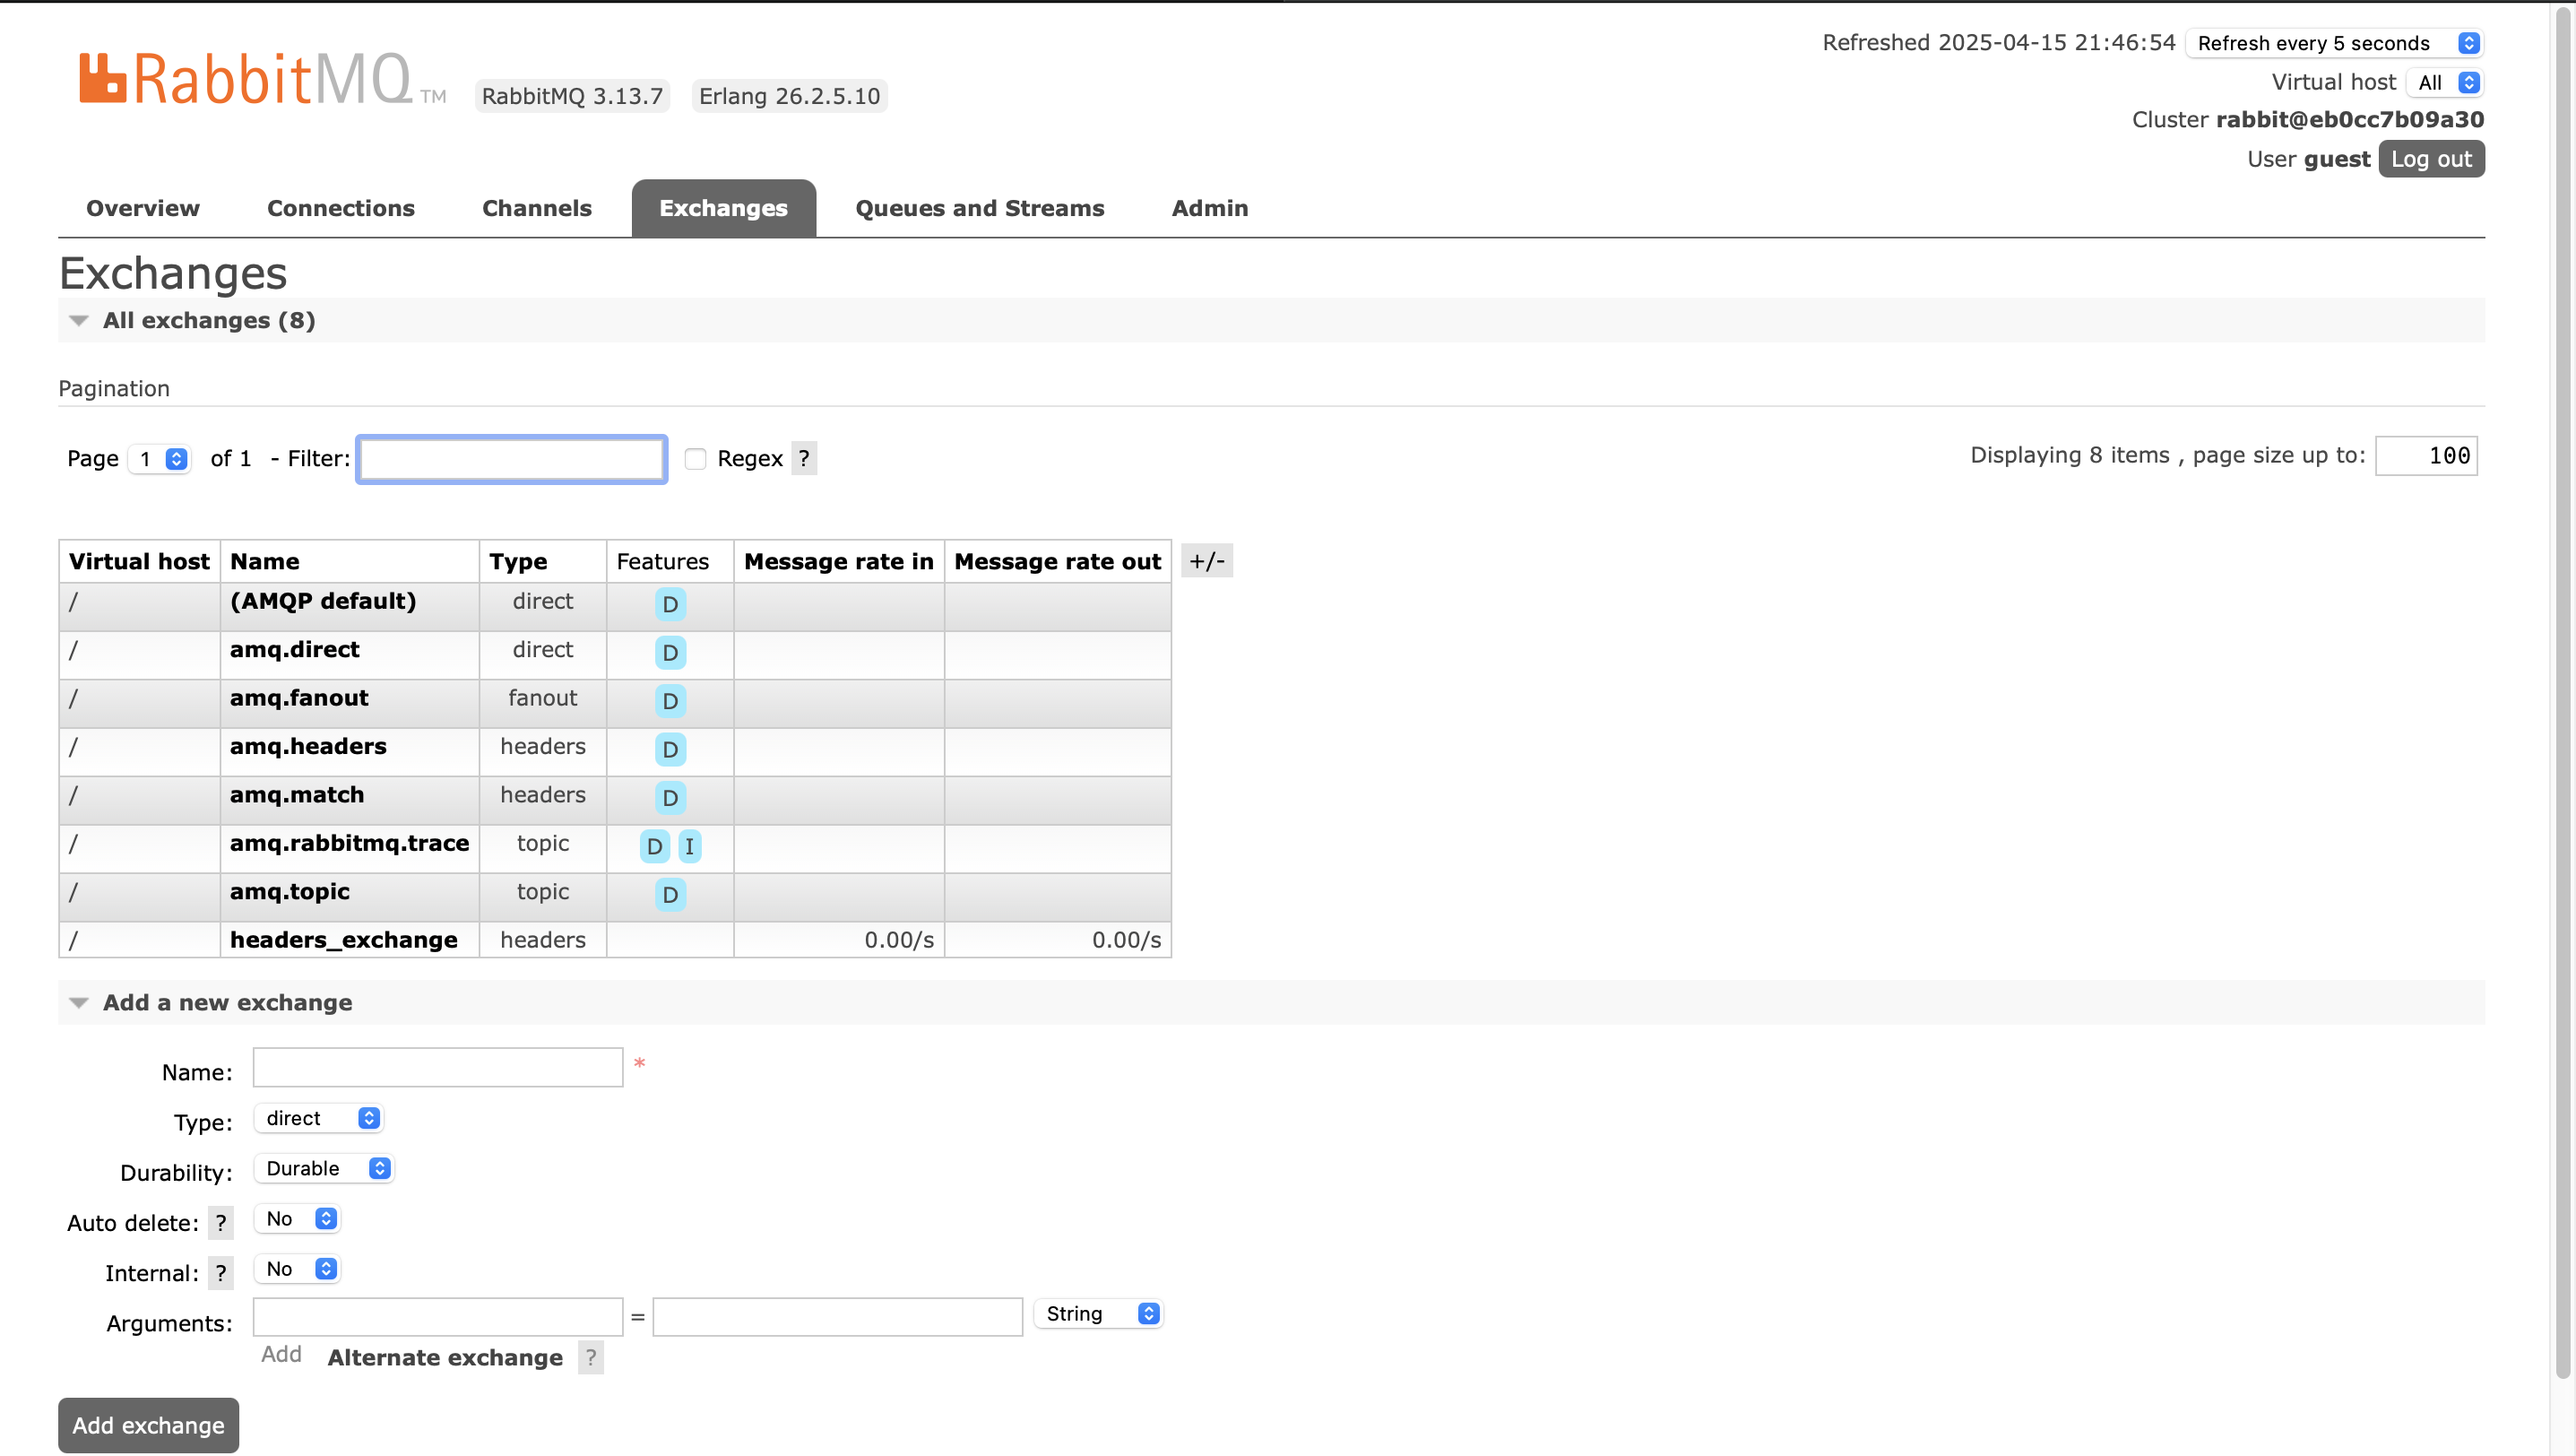
\includegraphics[width=0.7\textwidth]{Exchanges.png}
	\caption{Exchanges RabbitMQ}
	\label{fig:syntdiag}
\end{figure}

\begin{figure}[H]
	\centering
	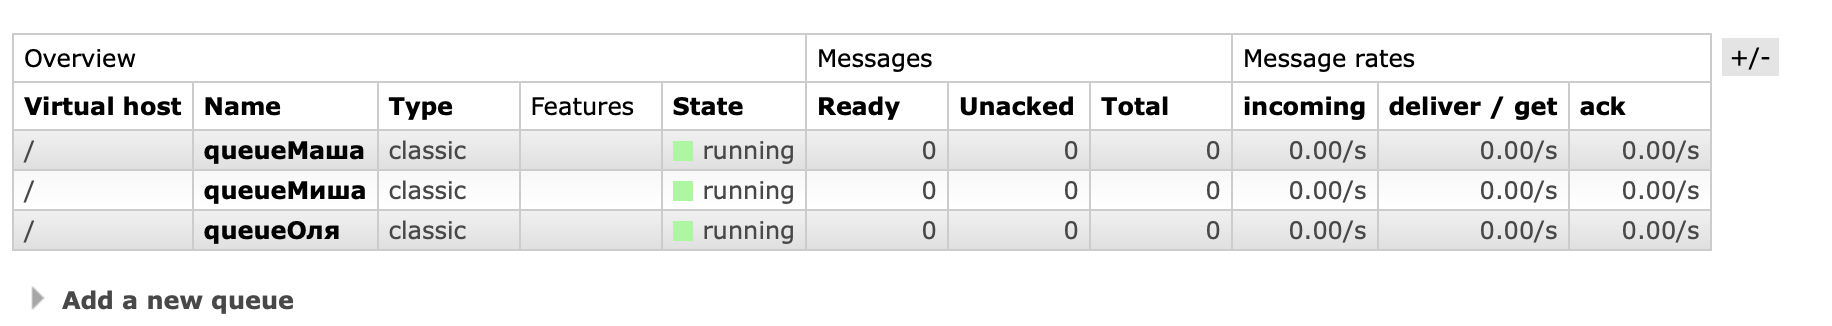
\includegraphics[width=0.7\textwidth]{q.png}
	\caption{Очереди}
	\label{fig:syntdiag}
\end{figure}

\begin{figure}[H]
	\centering
	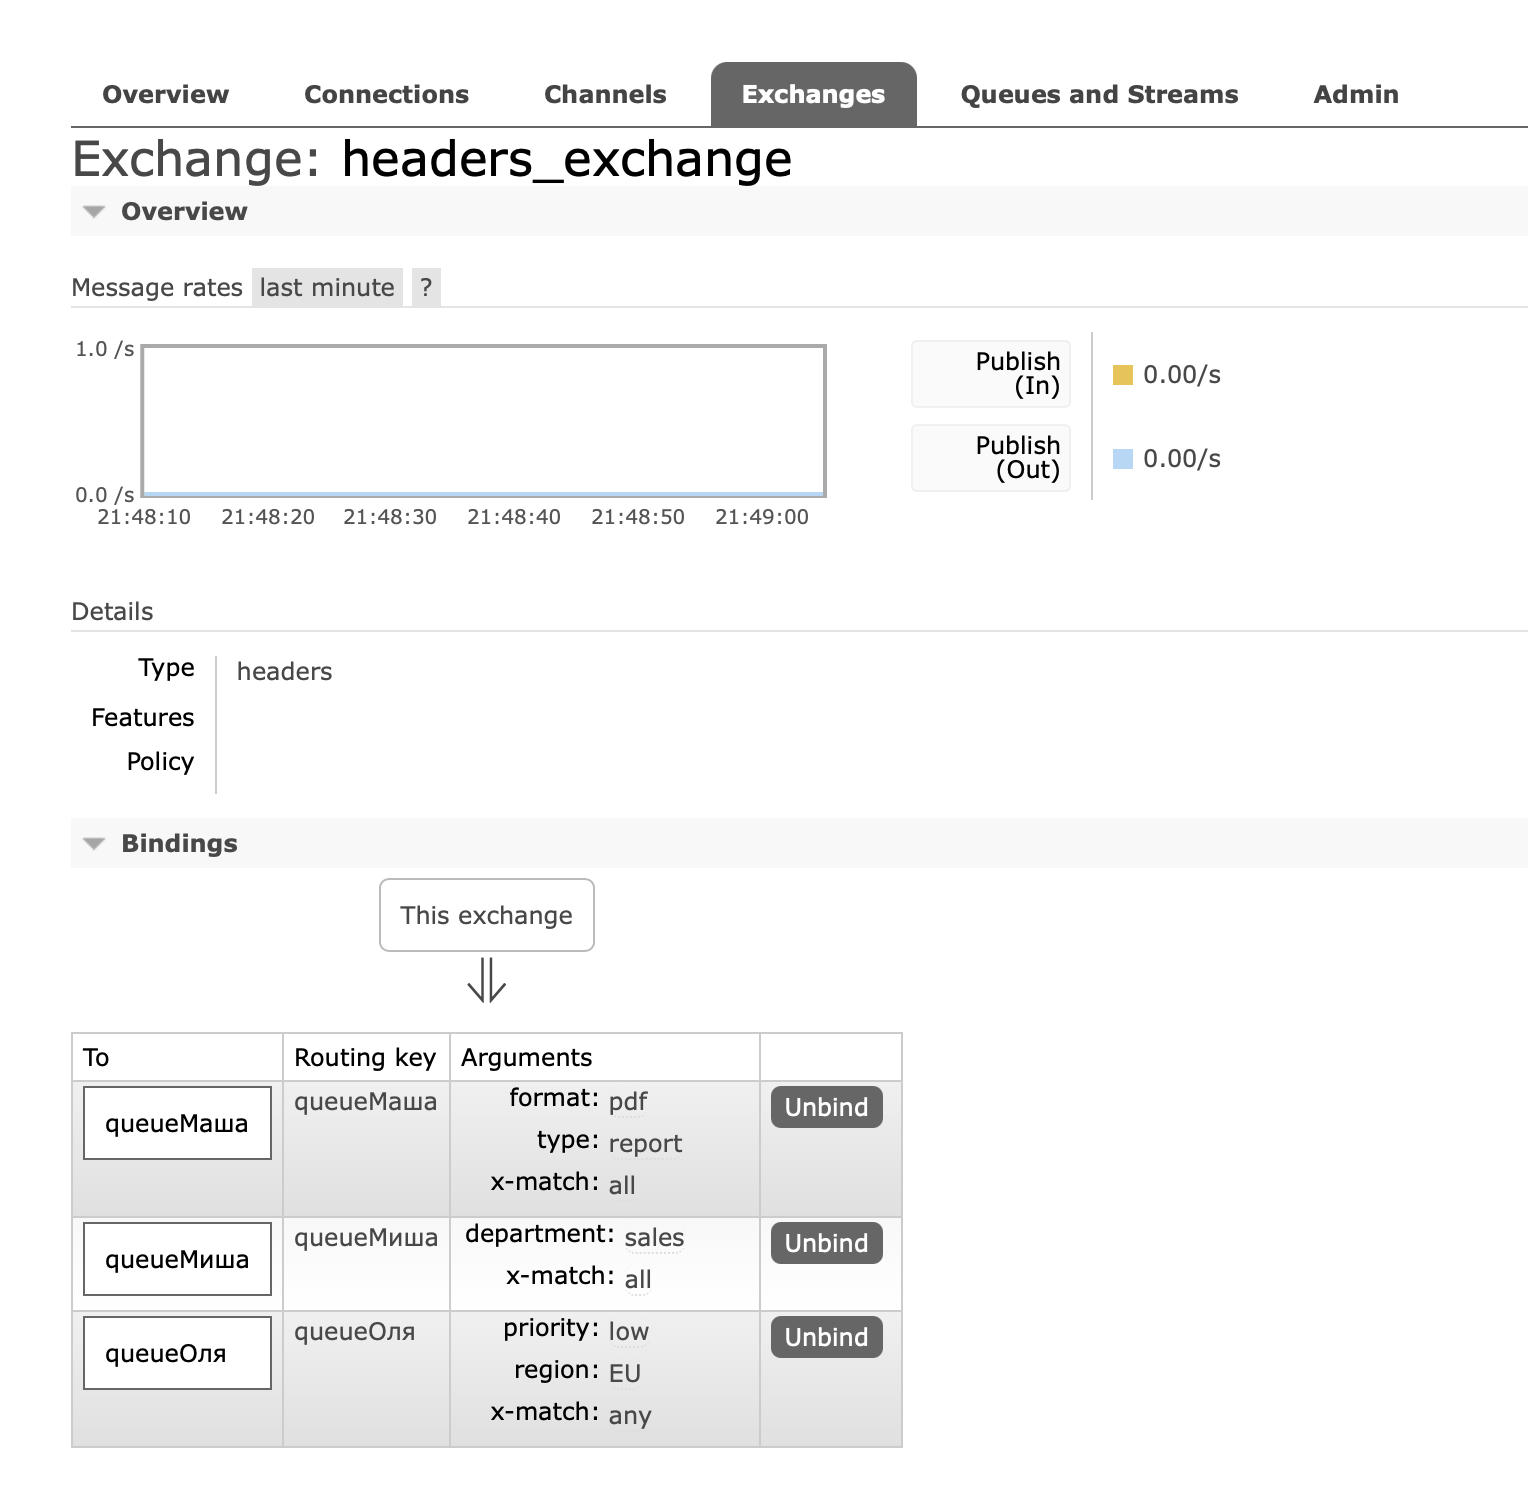
\includegraphics[width=0.7\textwidth]{HeadersExchange.png}
	\caption{Headers Exchange RabbitMQ}
	\label{fig:syntdiag}
\end{figure}

\newpage
\section*{Заключение}
\addcontentsline{toc}{section}{Заключение}
В результате этой работы были созданы Docker-контейнеры, реализующие схему передачи
между ними сообщений с использованием очереди RabbitMQ, и было показано как именно
осуществляется передача в этих условиях.
Контейнеры были связаны между собой с помощью Docker Compose.

\newpage
\section*{Список источников}
\addcontentsline{toc}{section}{Список источников}
\begin{enumerate}
	\item {[Электронный ресурс]. - URL:
	\url{https://docs.docker.com/engine/install/fedora/#install-
	using-the-repository} (дата обращения: 14.04.2024).}
	\item Introduction to Pika - Continuation-Passing Style [Электронный ресурс]. - URL: \url{https://pika.readthedocs.io/en/stable/intro.html?highlight=continuation#continuation-
	passing-style} (дата обращения: 12.04.2024).
	\item RabbitMQ tutorial — Topics [Электронный ресурс]. - URL: \url{https://www.rabbitmq.com/
	tutorials/tutorial-five-python} (дата обращения: 14.04.2025).
\end{enumerate}
\end{document}